\documentclass{beamer}

%\useoutertheme[glossy]{wuerzburg}
\useinnertheme[shadow,outline]{chamfered}
%\usecolortheme{shark}
\usecolortheme{beaver}
\beamertemplatenavigationsymbolsempty

\usefonttheme{professionalfonts}
\let\digamma\relax
\usepackage[scale=0.85,stdmathitalics=true,romanfamily=casual]{lucimatx}
\usefonttheme[stillsansseriftext]{serif}



\usepackage{fancyvrb}

%% Fancy syntax coloring via pygments
\usepackage{minted}
\definecolor{bg}{rgb}{0.95,0.95,0.95}
\usemintedstyle{borland}


\newenvironment{Rcode}
{\VerbatimEnvironment
 \begin{minted}[fontsize=\scriptsize,baselinestretch=1]{r}}%
{\end{minted}}

\newenvironment{Pcode}
{\VerbatimEnvironment
 \begin{minted}[fontsize=\scriptsize,baselinestretch=1]{python}}%
{\end{minted}}

\newenvironment{Code}[1]
{\VerbatimEnvironment
 \begin{minted}[fontsize=\scriptsize,baselinestretch=1]{#1}}%
{\end{minted}}


\usepackage{textfit} % commands \scaletoheight{height}{text} and \scaletowidth{width}{text}

\usepackage{tikz}

\usepackage{tcolorbox}

\newtheorem{Alert}{Alert}
\newtheorem{Highlight}{Highlight}

\newcommand{\Species}[1]{{\rmfamily \itshape #1}}
\newcommand{\Real}{\ensuremath{\mathbb{R}}}
\newcommand{\RealN}{\ensuremath{\mathbb{R}^n}}
\newcommand{\RealP}{\ensuremath{\mathbb{R}^p}}
\newcommand{\Mtx}[1]{\ensuremath{\mathbf{#1}}}
\newcommand{\Inv}[1]{\ensuremath{#1^{-1}}}
\newcommand{\InvMtx}[1]{\ensuremath{\mathbf{#1}^{-1}}}
\newcommand{\Red}[1]{\textcolor{red}{#1}}
\newcommand{\PsInv}[1]{\ensuremath{\mathbf{#1}^{+}}}

\usepackage{booktabs}



% --- Macro \xvec
% From a tex.stackexchange.com answer by Todd Lehman
% http://tex.stackexchange.com/questions/44017/dot-notation-for-derivative-of-a-vector
\makeatletter
\newlength\xvec@height%
\newlength\xvec@depth%
\newlength\xvec@width%
\newcommand{\xvec}[2][]{%
  \ifmmode%
    \settoheight{\xvec@height}{$#2$}%
    \settodepth{\xvec@depth}{$#2$}%
    \settowidth{\xvec@width}{$#2$}%
  \else%
    \settoheight{\xvec@height}{#2}%
    \settodepth{\xvec@depth}{#2}%
    \settowidth{\xvec@width}{#2}%
  \fi%
  \def\xvec@arg{#1}%
  \def\xvec@dd{:}%
  \def\xvec@d{.}%
  \raisebox{.2ex}{\raisebox{\xvec@height}{\rlap{%
    \kern.05em%  (Because left edge of drawing is at .05em)
    \begin{tikzpicture}[scale=1]
    \pgfsetroundcap
    \draw (.05em,0)--(\xvec@width-.05em,0);
    \draw (\xvec@width-.05em,0)--(\xvec@width-.15em, .075em);
    \draw (\xvec@width-.05em,0)--(\xvec@width-.15em,-.075em);
    \ifx\xvec@arg\xvec@d%
      \fill(\xvec@width*.45,.5ex) circle (.5pt);%
    \else\ifx\xvec@arg\xvec@dd%
      \fill(\xvec@width*.30,.5ex) circle (.5pt);%
      \fill(\xvec@width*.65,.5ex) circle (.5pt);%
    \fi\fi%
    \end{tikzpicture}%
  }}}%
  #2%
}
\makeatother

% --- Override \vec with an invocation of \xvec.
\let\stdvec\vec
\renewcommand{\vec}[1]{\xvec[]{#1}}
% --- Define \dvec and \ddvec for dotted and double-dotted vectors.
\newcommand{\dvec}[1]{\xvec[.]{#1}}
\newcommand{\ddvec}[1]{\xvec[:]{#1}}


\usepackage{pifont}
\newcommand{\weblink}{\ding{43}}  % hand with pointing finger

\definecolor{links}{HTML}{2A1B81}
\hypersetup{colorlinks,linkcolor=,urlcolor=magenta}

\usepackage{pdfpages}

\parskip=0.5em

%===========================================================
% Title Info
\title{Scientific Computing for Biologists}
\subtitle{Lecture 10: Mixture Models and Multi-dimensional Scaling} % (optional)

\author{Instructor: Paul M. Magwene}
\date{05 November 2013}


\begin{document}

\begin{frame}
\titlepage
\end{frame}



%===========================================================
\begin{frame}
  \frametitle{Outline of Lecture}

\begin{itemize}
    \item Mixture model based clustering
    \item Multi-dimensional scaling (MDS)
\end{itemize}

\end{frame}



%===========================================================
\begin{frame}
  \frametitle{Clustering with Mixture Models}

\begin{block}{Goal}
Method for assigning observations to clusters and estimating parametric distributions that describe the clusters.
\end{block}

    Assume that the data set represents observations drawn from a mixture of $g$ sub-distributions (user specifies $g$), and that the probability density function of the mixture is given by:

\[
p_{\mathrm{mix}} = \sum_{s=1}^g \pi_s p(\Mtx{x};\Mtx{\theta}_s)
\]

Where the $p(\Mtx{x};\Mtx{\theta}_s)$ represents the $s$-th `component density' (sub-distributions) and the $\Mtx{\theta}_s$ are the component parameters.  The $\pi_s$ represent the weighting factor of the $s$-th component in the mixture.

\end{frame}
%===========================================================

%===========================================================
% Pull in slides from PDF
{
\setbeamercolor{background canvas}{bg=}

\includepdf[pages=14]{li-mixtures-lecture.pdf}
}
%===========================================================

%===========================================================
\begin{frame}
  \frametitle{Gaussian Mixture Models}

A common starting point in mixture modeling is to assume that the components are Gaussian.

If the data are univariate, then the mixture model is given by:

\[
p_{\mathrm{mix}} = \sum_{s=1}^g \pi_s f(\Mtx{x}|\mu_i, \sigma_i^2)
\]

where the $\mu_i$ and $\sigma_i$ are the means and standard deviations of each component distribution and:

\[
f(\Mtx{x}|\mu, \sigma) = \frac{1}{\sqrt{2\pi\sigma^2}}e^{-\frac{(x-\mu)^2}{2\sigma^2}}
\]

\end{frame}

%===========================================================


%===========================================================
\begin{frame}
  \frametitle{Example: Waiting time between Old Faithful eruptions}

\begin{center}
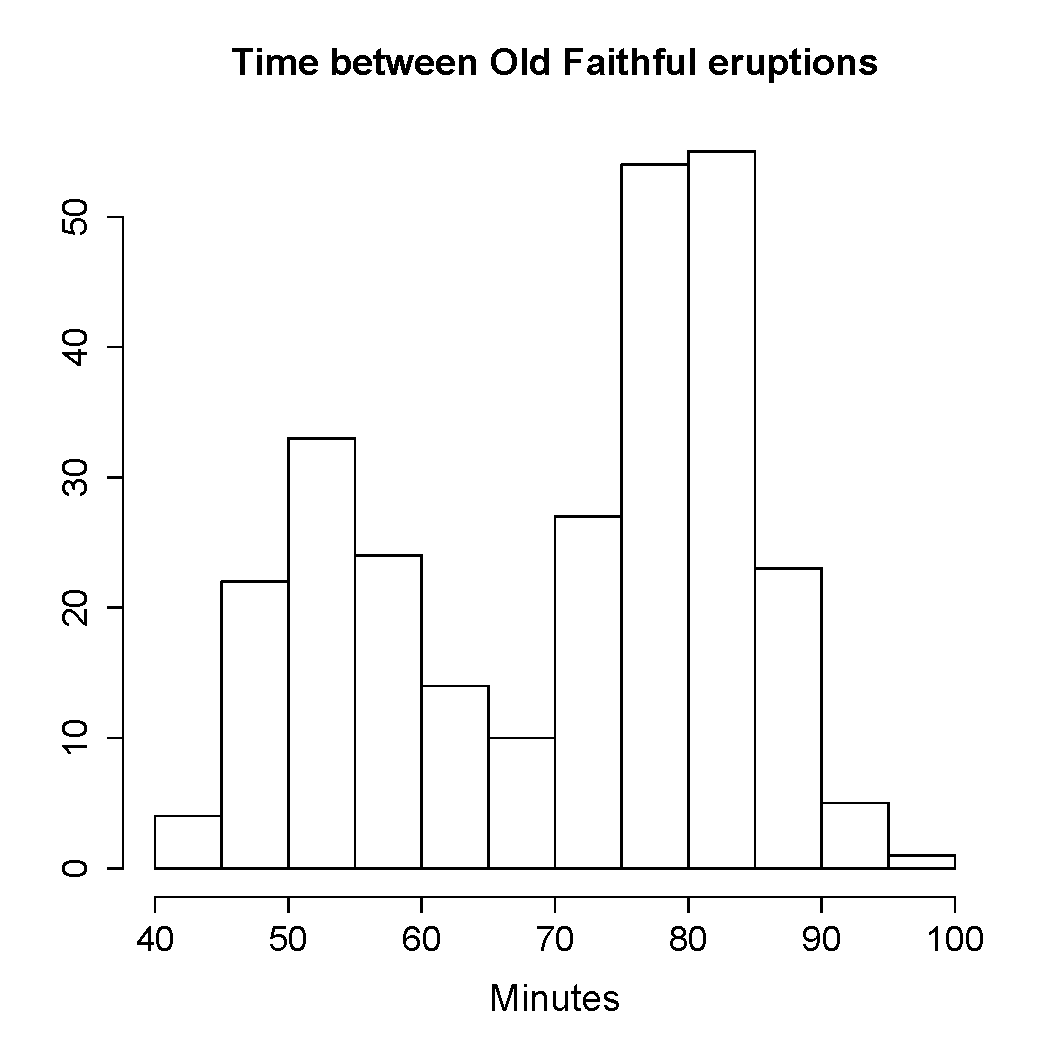
\includegraphics[height=3.1in]{waitingtime.pdf}
\end{center}

\end{frame}
%===========================================================

%===========================================================
\begin{frame}
  \frametitle{Example: Gaussian fit, Old Faithful waiting time}

\vspace*{-0.15in}
\begin{columns}
\begin{column}{7cm}
\begin{center}
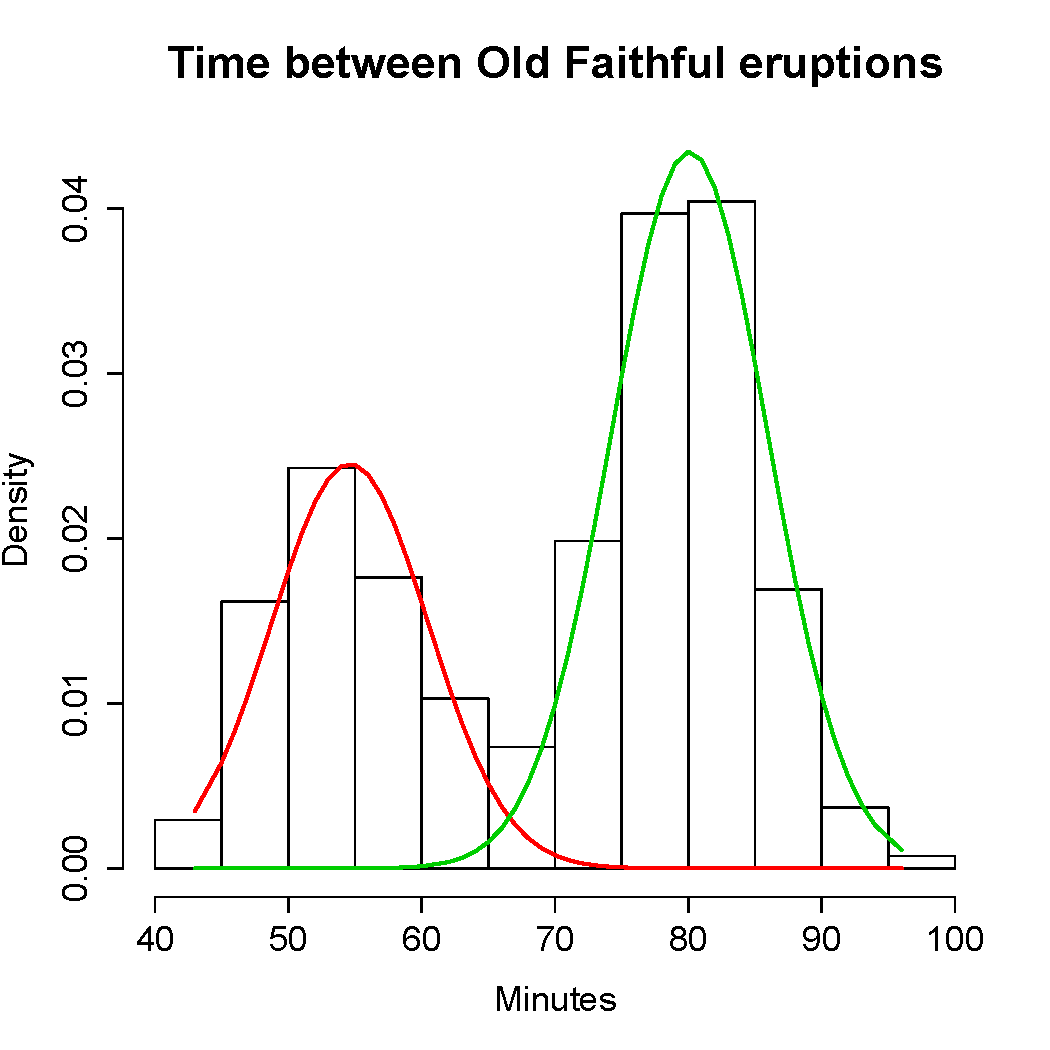
\includegraphics[height=3in]{waiting-fit.pdf}
\end{center}
\end{column}


\begin{column}{5cm}
\begin{eqnarray*}
\pi = (0.36, 0.64)\\
\mu = (54.6, 80.1)\\
\sigma = (5.87, 5.87)
\end{eqnarray*}
\end{column}

\end{columns}



\end{frame}
%===========================================================





%===========================================================
\begin{frame}
  \frametitle{Gaussian Mixture Models, Multivariate data}

When the components are multivariate Gaussian distributions:

\[
N(\Mtx{x};\Mtx{\theta}) \equiv (2\pi)^{-D/2}|\Sigma|^{-1/2} \exp
\left[
-\frac{1}{2}(\Mtx{x}-\Mtx{\mu})^{T} \Sigma^{-1} - (\Mtx{x}-\Mtx{\mu})
\right]
\]

each with a different mean vector, $\Mtx{\mu}$ ($\Mtx{\mu} \in \Real^p$), and covariance matrix, $\Sigma$ ($p \times p$).

\end{frame}
%===========================================================

%===========================================================
\begin{frame}
\frametitle{Mixture Model Clustering, Example}
\begin{center}
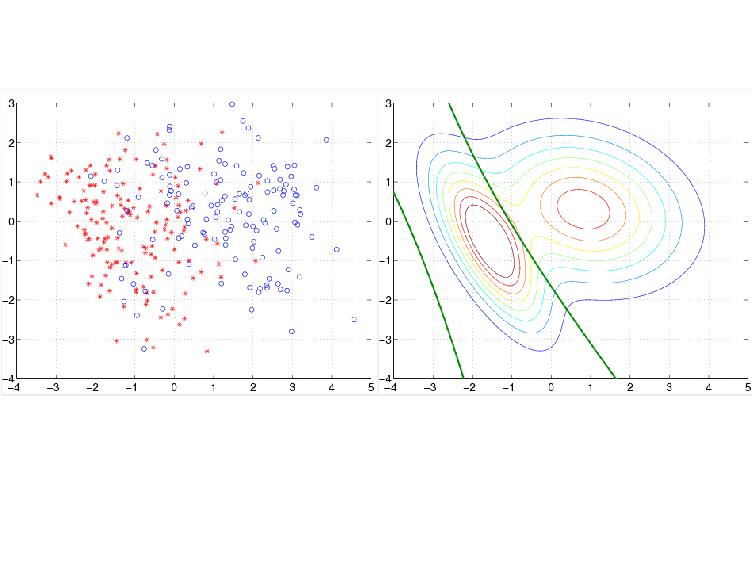
\includegraphics[width=\textwidth]{heart-disease.pdf}
\end{center}

Heart disease example: 297 samples (137 with heart disease). 13 quantitative varibles (e.g. cholesterol, max heart rate, etc). Data centered and normalized. Data projected onto first two PCs. Two-component Gaussian mixture fit.

\end{frame}
%===========================================================


%===========================================================
\begin{frame}
  \frametitle{How do we `solve' the mixture model problem?}

The mixture model problem involves optimization over multiple parameters.

The standard approach to estimating the parameters is called the "Expectation-Maximization" (EM) algorithm.

\begin{itemize}
    \item Described by Dempster, Laird, and Rubin (1977)
    \item Provides a way to iterative compute a maximum likelihood estimation when the observed data are incomplete or there are `latent' parameters.
\end{itemize}


\end{frame}
%===========================================================

%===========================================================
\begin{frame}
  \frametitle{Overview of the EM Algorithm}

\begin{enumerate}
    \item Guess a set of starting parameters
    \item Use these starting parameters to `estimate' the complete data
    \item Use the estimates of the complete data to update the parameters
    \item Repeat steps 2 and 3 until convergence
\end{enumerate}

\end{frame}
%===========================================================



%===========================================================
% Pull in slides from PDF
% {
% \setbeamercolor{background canvas}{bg=}
% 
\includepdf[pages=24]{li-mixtures-lecture.pdf}
}
%===========================================================

%===========================================================
\begin{frame}[plain,c]
\begin{center}
\Huge Multidimensional Scaling
\end{center}
\end{frame}
%===========================================================



%===========================================================
\begin{frame}
  \frametitle{Multidimensional Scaling (MDS)}

\begin{block}{Goal}
Given dissimilarities between objects, $d_{ij}$, estimate a $k$-dimensional set of points, \Mtx{X}, such that $|x_i - x_j| \approx d_{ij}$.
\end{block}


\end{frame}
%===========================================================

%===========================================================
\begin{frame}[shrink=5]
\frametitle{Derivation of MDS}

\begin{block}{Motivation}
    If we know the coordinates of $n$ points in $p$-dimensional space, we can easily calculate the Euclidean distances between every pair of points. \alert{Can we reverse this process, starting with the distances and getting back the coordinates points?}
\end{block}

Consider a data matrix \Mtx{X} ($n \times p$).  Let  $\Mtx{Q} = \Mtx{X}\Mtx{X}'$ be a $n \times n$ matrix, where
\[
q_{rs} = \sum_{j=1}^p x_{rj}x_{sj}
\]

If $d_{rs}^2$ is the squared Euclidean distance between points $r$ and $s$ then we can write this as:
\begin{eqnarray*}
d_{rs}^2 &=& \sum_{j=1}^p (x_{rj}-x_{sj})^2 \\
         &=& q_{rr} + q_{ss} - 2q_{rs}
\end{eqnarray*}

\end{frame}
%===========================================================

%===========================================================
\begin{frame}[shrink=5]
\frametitle{Derivation of MDS, cont.}

With a little bit of simple algebra we can show that:
\[
q_{rs} = -\frac{1}{2}(d_{rs}^2- d_{r.}^2 - d_{.s}^2 - d_{..}^2)
\]

where a dot represent the average of values over the corresponding suffix: $d_{r.}^2$ is the average over the $r$th row of matrix $\Mtx{D}=(d_{ij}^2)$, $d_{.s}^2$ is the average over the $s$th column of \Mtx{D}, and $d_{..}^2$ is the average of all elements of \Mtx{D}.So, given \Mtx{D}, the squared interpoint distances, we can regenerate \Mtx{Q}.

Since \Mtx{Q} is symmetric, we can use eigendecomposition to write $\Mtx{Q}=\Mtx{T}\Mtx{\Lambda}\Mtx{T}'$  where $\Mtx{\Lambda}$ is a diagonal matrix of eigenvalues of \Mtx{Q} and \Mtx{T} is the matrix of eigenvectors. Furthermore we can write $\Mtx{Q}=\Mtx{T}\Mtx{\Lambda}\Mtx{T}'=\Mtx{T}\Mtx{\Lambda}^{\frac{1}{2}}\Mtx{\Lambda}^{\frac{1}{2}}\Mtx{T}'= \Mtx{X}\Mtx{X}'$ where $\Mtx{X}=\Mtx{T}\Mtx{\Lambda}^{\frac{1}{2}}$.

\alert{Thus we've found how to get \Mtx{X} from the squared distances.}

{\footnotesize See Krzanowski, W.\ J. (2000) Principles of multivariate analysis, for full details.}
\end{frame}
%===========================================================

%===========================================================
\begin{frame}
\frametitle{Algorithm for MDS}

Given an $n \times n$ matrix of dissimilarities, $\Mtx{D}$, with elements $d_{ij}$:

\begin{enumerate}
\item Form matrix, $\Mtx{E}$, where $e_{ij} = -\frac{1}{2} d_{ij}^2$

\item Subtract from each element of $\Mtx{E}$ the means of the row and column in which it is located and the mean of all elements of $\Mtx{E}$; call the resulting matrix $\Mtx{F}$

\item Calculate the eigenvalues ($\lambda_i$) and eigenvectors $\Mtx{v}_i$ of $\Mtx{F}$, sorted in decreasing order. Eigenvectors should be normalized (i.e. $\Mtx{v}_i \cdot \Mtx{v}_i = 1$).

\item The coordinates of the $n$ point on the $j$-th axis are given $\sqrt{\lambda_j}\Mtx{v}_j$

\end{enumerate}

\end{frame}
%===========================================================

%===========================================================
\begin{frame}
  \frametitle{Potential MDS Complications}

If the $d_{ij}$ are metric (i.e. $d_{ij} \leq d_{ik} + d_{kj}$) than $\Mtx{F}$ is always positive semidefinite (psd; i.e. eigenvalues $\geq 0$).

\medskip
If $\Mtx{F}$ is not psd than how do you handle negative eigenvalues?

\begin{itemize}

\item Most common approach is only to consider positive eigenvalues
\item This is OK if negative eigenvalues have small magnitude
\item If negative eigenvalues are large than approximation tends to be poor

\end{itemize}


\end{frame}
%===========================================================

%===========================================================
\begin{frame}
  \frametitle{Multidimensional Scaling: Keep in mind...}

\begin{itemize}
\item The configuration produced by any MDS method is indeterminate with respect to translation, rotation, and reflection.

\end{itemize}


\end{frame}
%===========================================================

%===========================================================
\begin{frame}
  \frametitle{Relationship between metric MDS and PCA}

 If the $d_{ij}$ are Euclidean distances from a data matrix, $\Mtx{X}$, then metric MDS of $\Mtx{D}$ yields the PC scores obtained by PCA of $\Mtx{X}$.

 \medskip
  \begin{block}{Interpretation}
PCA and MDS are dual methods:
\begin{itemize}
  \item One operates on variable space (PCA)
  \item The other operates on subject space (MDS)
\end{itemize}
\end{block}

\end{frame}
%===========================================================

%===========================================================
\begin{frame}
  \frametitle{Other Metric MDS Approaches}

\begin{itemize}
\item Classical MDS minimizes:
\[
\sum_i \sum_j(\delta_{ij}^2 - d_{ij}^2)
\]

where $\delta_{ij}$ is the distance between observations $i$ and $j$ in the MDS approximation.

\item Alternates approaches try to minimize other measures of discrepancy. For example, ``Sammon MDS" minimizes:
\[
\sum_i \sum_j (\delta_{ij} - d_{ij})^2
\]
\end{itemize}
\end{frame}
%===========================================================

%===========================================================
\begin{frame}
  \frametitle{Non-Metric MDS}

Non-metric MDS approaches try to preserve only the rank order of the distances.

If
\[
d_{i1,j1} < d_{i2,j2} < \cdots< d_{im,jm}
\]

then
\[
\delta_{i1,j1} < \delta_{i2,j2} < \cdots< \delta_{im,jm}
\]

Shepard-Kruskal solution:

\begin{itemize}
\item Find $\hat{d}_{ij}$ that minimizes:
\[
\mbox{STRESS} = \sqrt{ \{ \frac{\sum \sum_{i < j}(d_{ij}-\hat{d}_{ij})^2 }{\sum \sum d_{ij}^2} \} }
\]
\end{itemize}

\bigskip

\end{frame}
%===========================================================

%===========================================================
\begin{frame}
  \frametitle{MDS Example: Road Distances}

Input $\Mtx{D}$: road distances between U.S. cities

\begin{center}
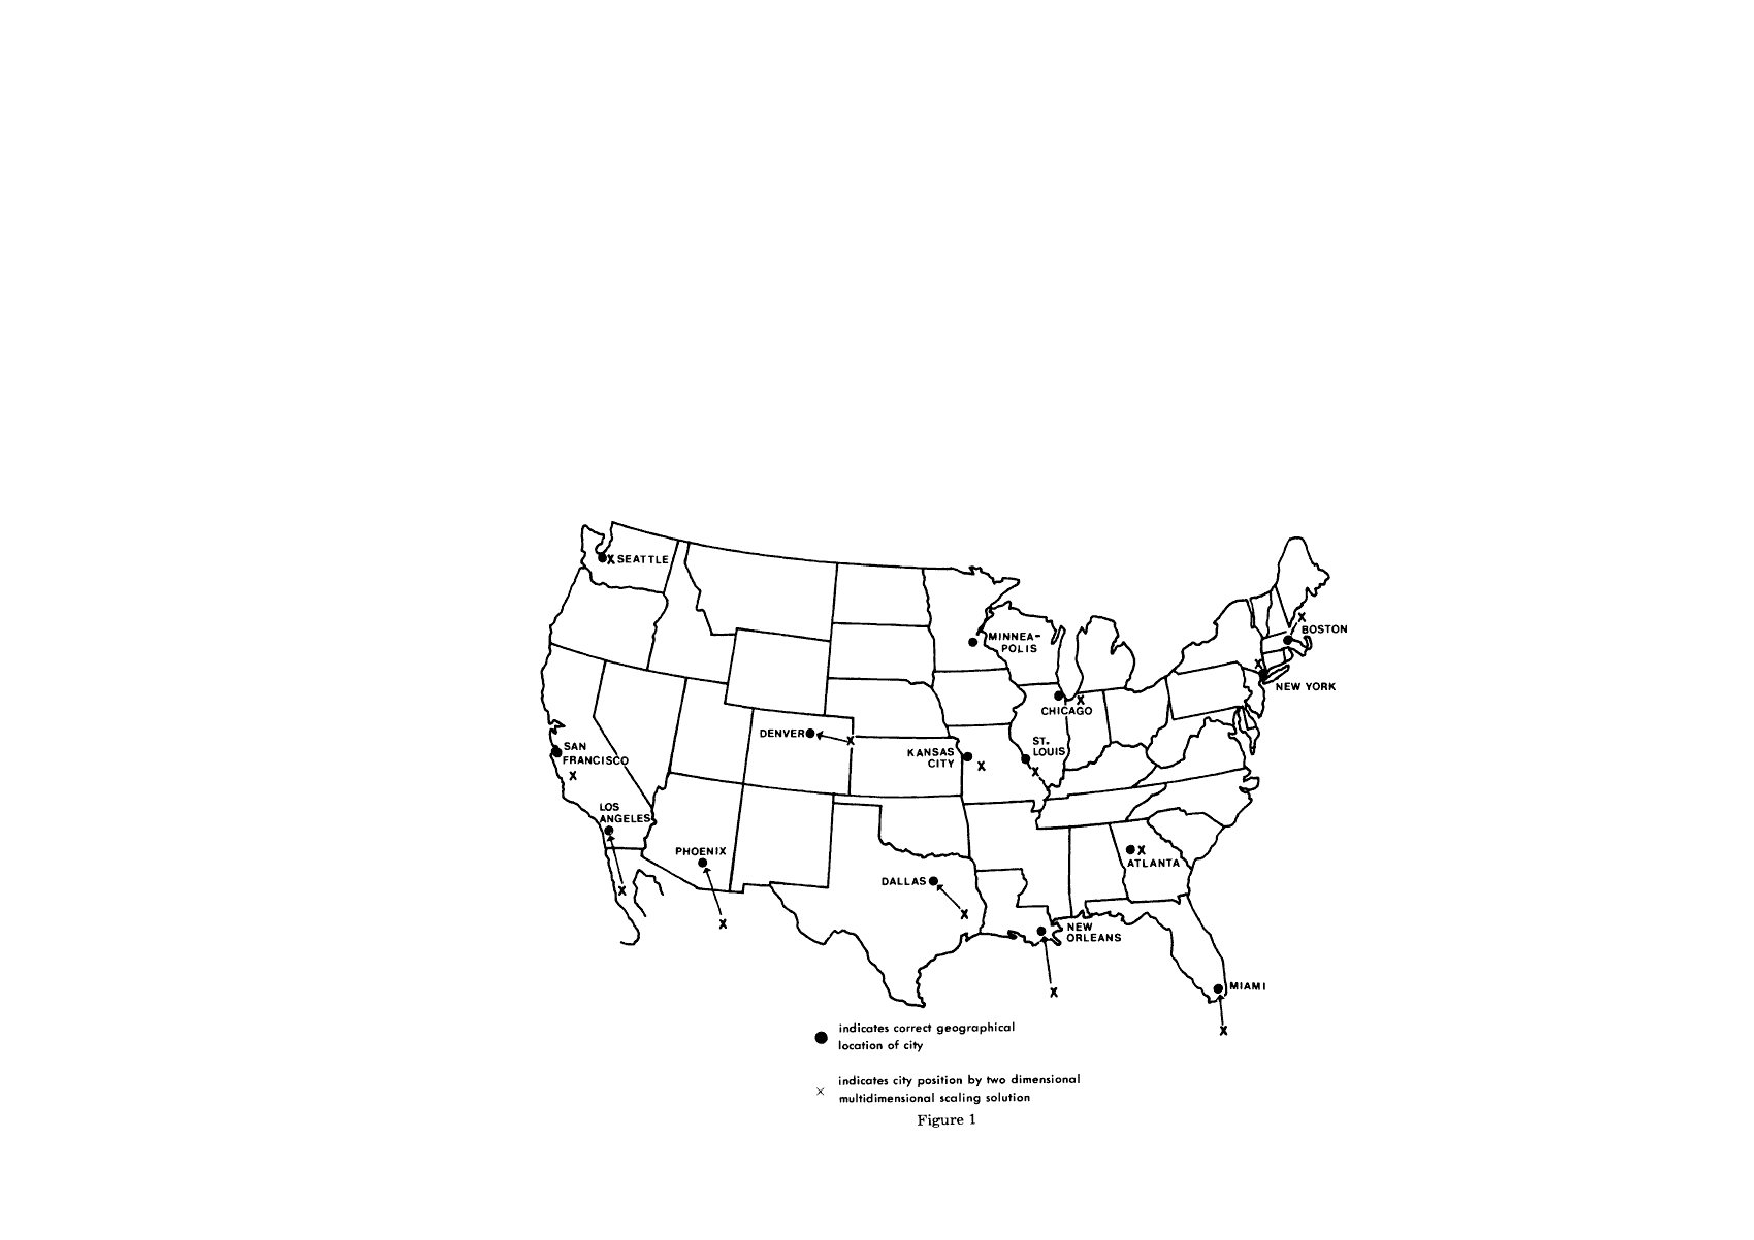
\includegraphics[height=2.9in]{mds-road}
\end{center}

\end{frame}
%===========================================================


%===========================================================
\begin{frame}[plain,c]
\begin{center}
\Huge Minimum Spanning Tree
\end{center}
\end{frame}
%===========================================================



%===========================================================
\begin{frame}
  \frametitle{Minimum Spanning Tree}

\begin{block}{Goal}
Construct a tree that connects all points in the data set and whose total length is minimized.
\end{block}

\emph{Statistical applications}
\begin{itemize}
    \item highlights close neighbors in a data set
    \item useful check for distortions produced by projection techniques
    \item tests of normality
\end{itemize}
\medskip

\emph{Other applications}
\begin{itemize}
    \item urban planning/engineering
    \item circuit design
\end{itemize}

\end{frame}
%===========================================================

%===========================================================
\begin{frame}
  \frametitle{Example Data Set}

\begin{center}
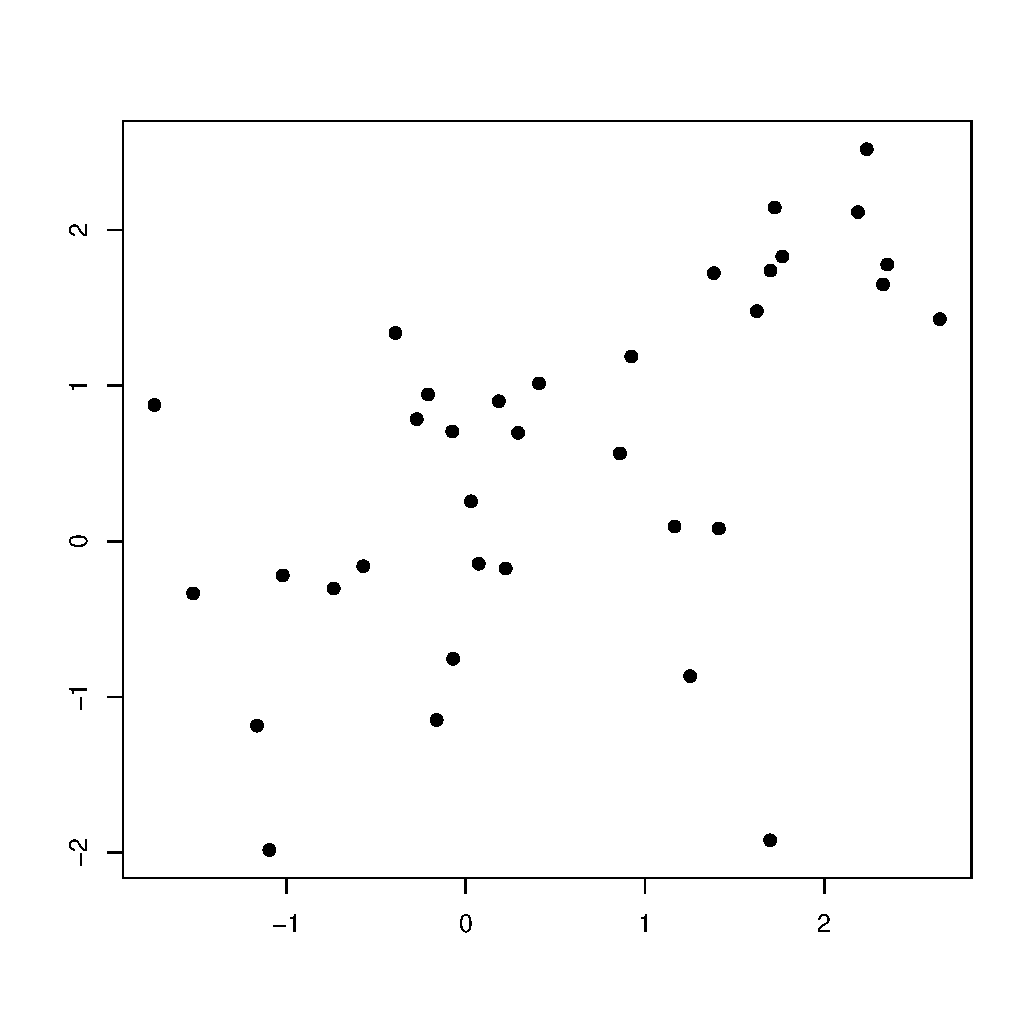
\includegraphics[height=3.1in]{points-only}
\end{center}
\end{frame}
%===========================================================

%===========================================================
\begin{frame}
  \frametitle{Minimum Spanning Tree: Example}

  
\begin{center}
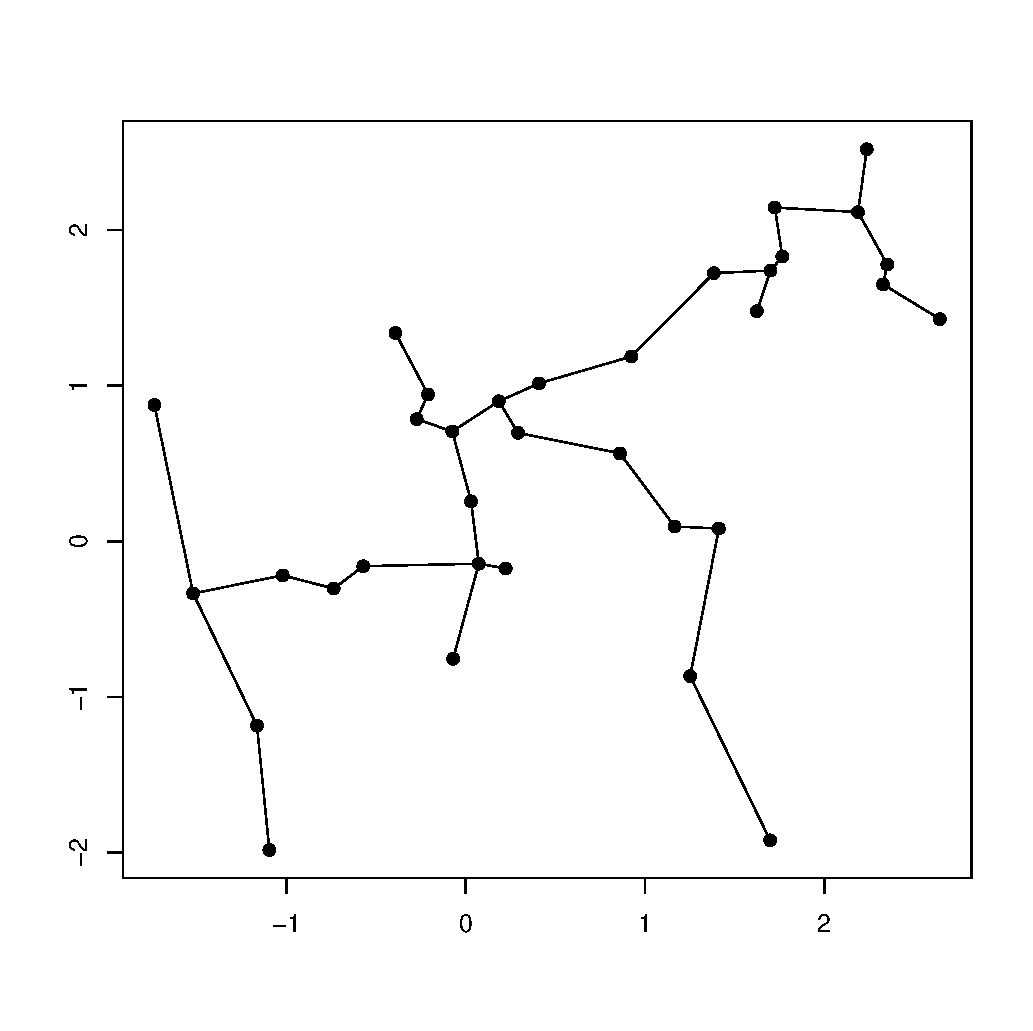
\includegraphics[height=3.1in]{points-mst}
\end{center}
\end{frame}
%===========================================================

%===========================================================
\begin{frame}
  \frametitle{Relationship between MST and Single Linkage Clustering}


\begin{itemize}

\item Cut a single linkage dendrogram at height, $\delta \dashrightarrow$ clusters

\item Remove all edges in the MST with length $\geq \delta \dashrightarrow$ subgraphs corresponding to the same clusters

\end{itemize}

\end{frame}
%===========================================================

%===========================================================
\begin{frame}
  \frametitle{A Generic MST Algorithm}


\textbf{Input}: dissimilarity matrix, \Mtx{D}, between each object (point) of interest
\begin{enumerate}
\item Create a graph, G, where  $V = \{v_1,\ldots,v_n\}$ and $E =\{\}$ ($E$ initially empty)
\item Find the smallest dissimilarity, $d_{ij}$ where (i,j) is not in $E$.
\item Add (i,j) to $E$ if (i,j) does not create a cycle
\item Repeat from step 2 until every vertex is included in at least one edge
\end{enumerate}

Not particularly efficient algorithm, but simple. More efficient algorithms for finding MSTs include Kruskal's Algorithm and Prim's algorithm.

\end{frame}
%===========================================================

%===========================================================
\begin{frame}
  \frametitle{Applications of the MST}

MST tends to highlight close neighbors; can be used to look for distortions associated with projections to lower dimensional spaces.

\begin{block}{Using the MST to look for Projection Distortion}
\begin{itemize}
    \item  Calculate the MST based on dissimilarity in a high-dimensional space
    \item Draw the MST edges among points in the projection space (e.g. MDS or PCA)
    \item MST edges that cross highlight geometric relationships among points that are not well represented by the projection
\end{itemize}
\end{block}
\end{frame}
%===========================================================




\end{document}



%===========================================================
\begin{frame}
  \frametitle{XXX}

\end{frame}
%===========================================================

